\documentclass[
10pt,
%handout
]{beamer}

\mode<presentation> {\usetheme{Kaiping}}
\setbeamercovered{transparent} 

\usepackage[english]{babel}

\usepackage{fontspec}
\setmainfont{DejaVu Sans}
\setmonofont{DejaVu Sans Mono}
\setsansfont{DejaVu Sans}

\usepackage{multimedia}
\usepackage{media9}

\usepackage{xcolor}
\usepackage{graphicx}
\usepackage{tikz}
\usepackage{tikz-cd}

% \usepackage[style=authoryear]{biblatex}
\usepackage[backend=biber,
            bibstyle=biblatex-sp-unified,
            citestyle=sp-authoryear-comp,
            maxcitenames=2,url=false,
            footcite=footnote,
            maxbibnames=99]{biblatex}
\bibliography{/home/gereon/Downloads/My Library}

\usefonttheme[onlymath]{serif}
\usetheme{Warsaw}
\setbeamerfont{footnote}{size=\tiny}
\setbeamercovered{transparent}

\title{Network Phylogenies of Abui}
\subtitle{An initial look at inferring language contact}
\author{Gereon A. Kaiping}
\institute{Leiden University Centre for Linguistics, Niederlande}
\date{2019-08-21}

\begin{document}

\begin{frame}[plain]
  \titlepage
\end{frame}
\begin{frame}
  \tableofcontents
\end{frame}
\section{Network Phylogenies}
\begin{frame}{Why infer phylogenetic networks?}
  \begin{itemize}
  \item Language contact: important driver of language evolution
  \item Tree assumption in phylogenetics is limiting
    \begin{itemize}
    \item Dealing with borrowing as pre-cleanup is hard
    \item Language contact is part of the history to be inferred
    \end{itemize}
  \item Grouping word trees for understanding strata in the vocabulary
  \end{itemize}
\end{frame}
\begin{frame}{State of the art}
  \begin{itemize}
  \item Big bubble of Bayesian phylogenetics in linguistics, with slowly improving tools
  \item SplitsTrees, NeighborNets → No model, only visualization
  \item Initial bits of Bayesian network inference
  \end{itemize}
  Here: A (first?) practical look at network inference for languages
\end{frame}
\section{Abui}
\begin{frame}{Language sample: Abui}
  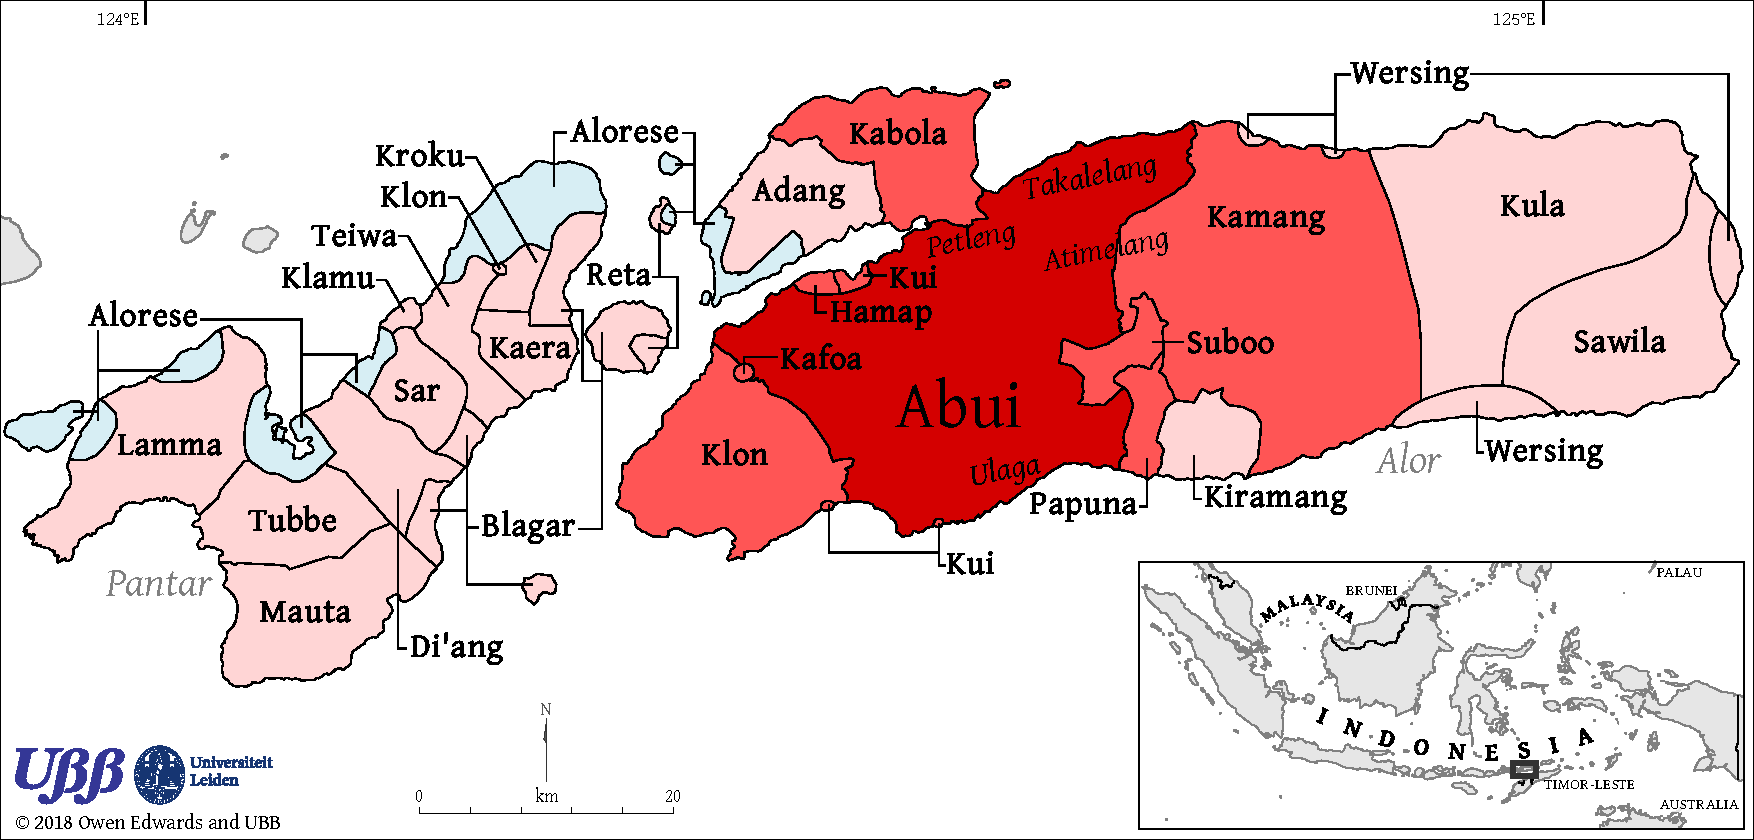
\includegraphics[width=\textwidth]{Abui_Neighbors}
\end{frame}
\section{Results}
\begin{frame}{Recipe}
  \begin{itemize}
  \item BEASTling\footcite{maurits2017beastling} configuration with rate variation
    \begin{itemize}
      \item Abui \& Neighbors
      \item Data from LexiRumah\footcite{lexirumahpaper} with ACD\footcite{list2012lexstat}
      \item pseudo-Dollo Covarion model\footcite{bouckaert2017pseudo}
    \end{itemize}
  \item Python script to add Species Network\footcite{zhang2018bayesian},
    grouping ‘gene’ trees
  \item Phylogenetic inference in BEAST\footcite{bouckaert2014beast}
  \end{itemize}
  Full analysis available under \url{http://github.com/Anaphory/abui-network}
\end{frame}
\begin{frame}{\uncover<-1>{Results}\visible<2->{Issues}}
  \begin{columns}
    \begin{column}{0.5\textwidth}
      \pause
      Practical issues
      \begin{itemize}
      \item SpeciesNetwork is buggy
        \pause
      \item SN takes only small data (genes, taxa)
        \pause
      \item Driver file construction is complicated
        \pause
      \item Displaying results
      \end{itemize}
      \pause
      Obvious issues
      \begin{itemize}
      \item How to summarize results? (!)
      \item How many trees to infer?
      \item How to improve the MCMC?
      \end{itemize}
    \end{column}
    \begin{column}{0.5\textwidth}
      \pause
      Theoretical issues
      \begin{itemize}
      \item Multispecies Network Coalescent prior: good?
      \item Population model?
      \item Convergence vs. local maximum?
      \item Non-lexical data?
      \item Calibrations?
      \item What amount of reticulation should be expect?
      \item Do we have extremely tree-like histories to test this on?
      \end{itemize}
    \end{column}
  \end{columns}
\end{frame}
\begin{frame}{Results}
  A typical (?) network\footnote{\url{https://icytree.org/}}
  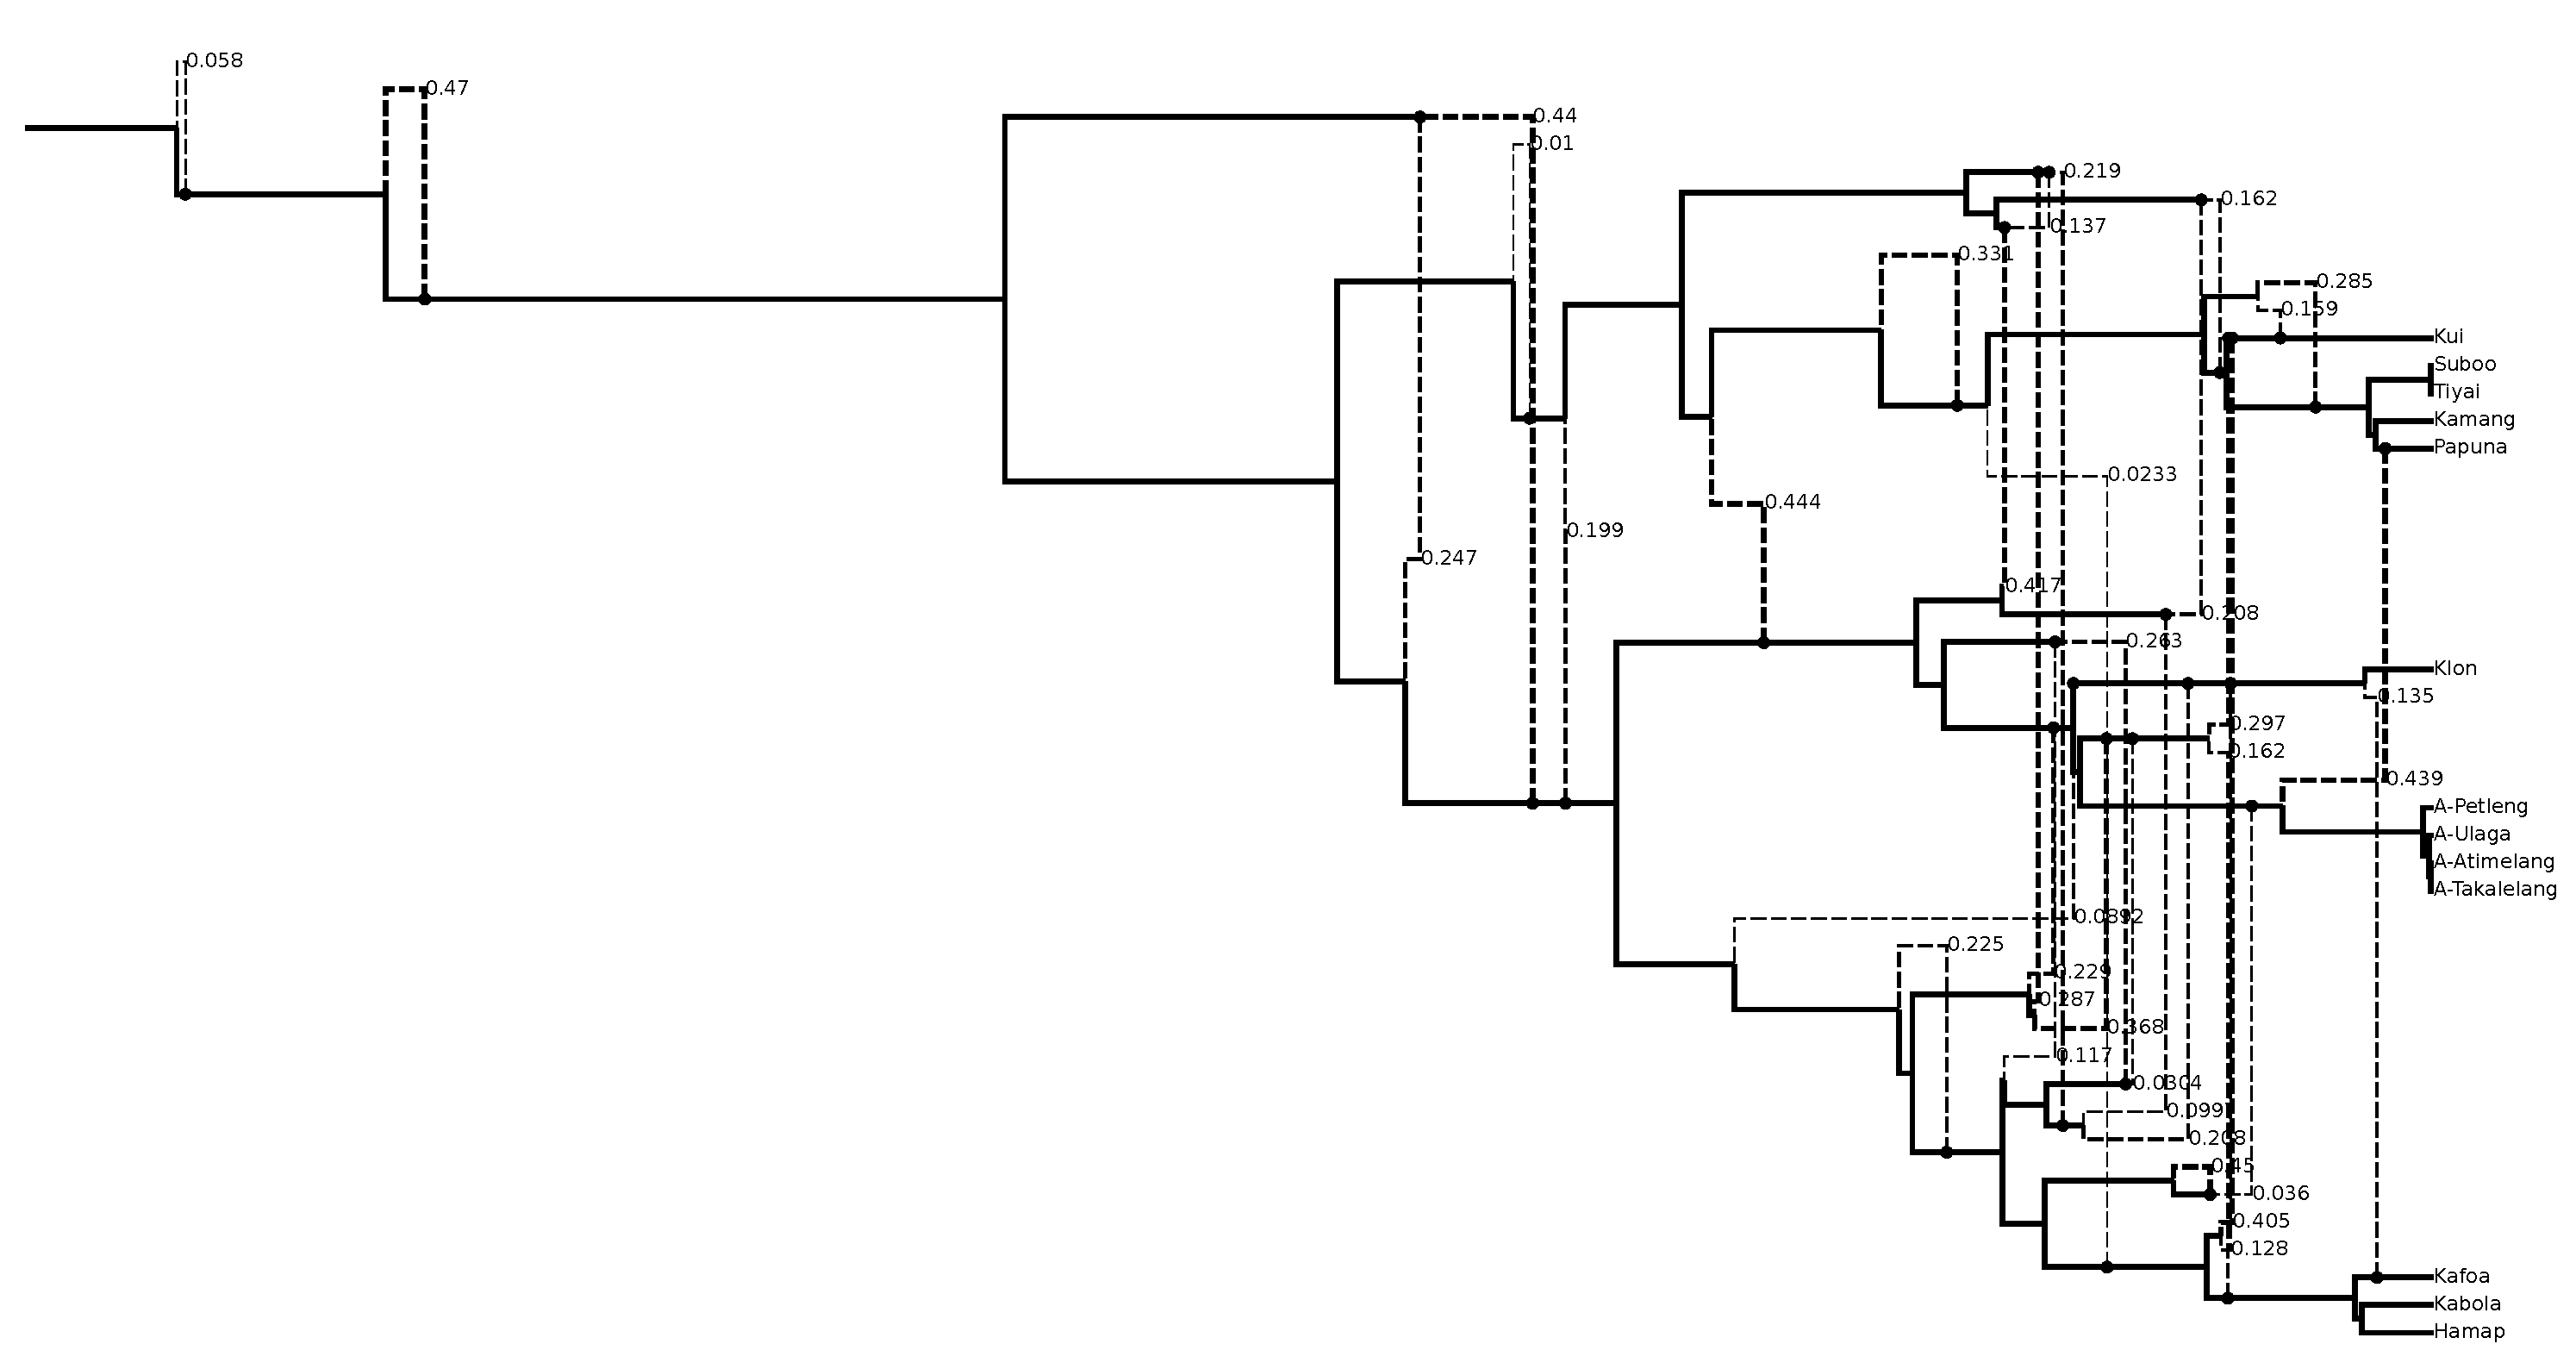
\includegraphics[width=\textwidth]{tree}
\end{frame}
\begin{frame}{Results}
  Summary of pairwise distances
  \begin{columns}
    \begin{column}{1.2\textwidth}
      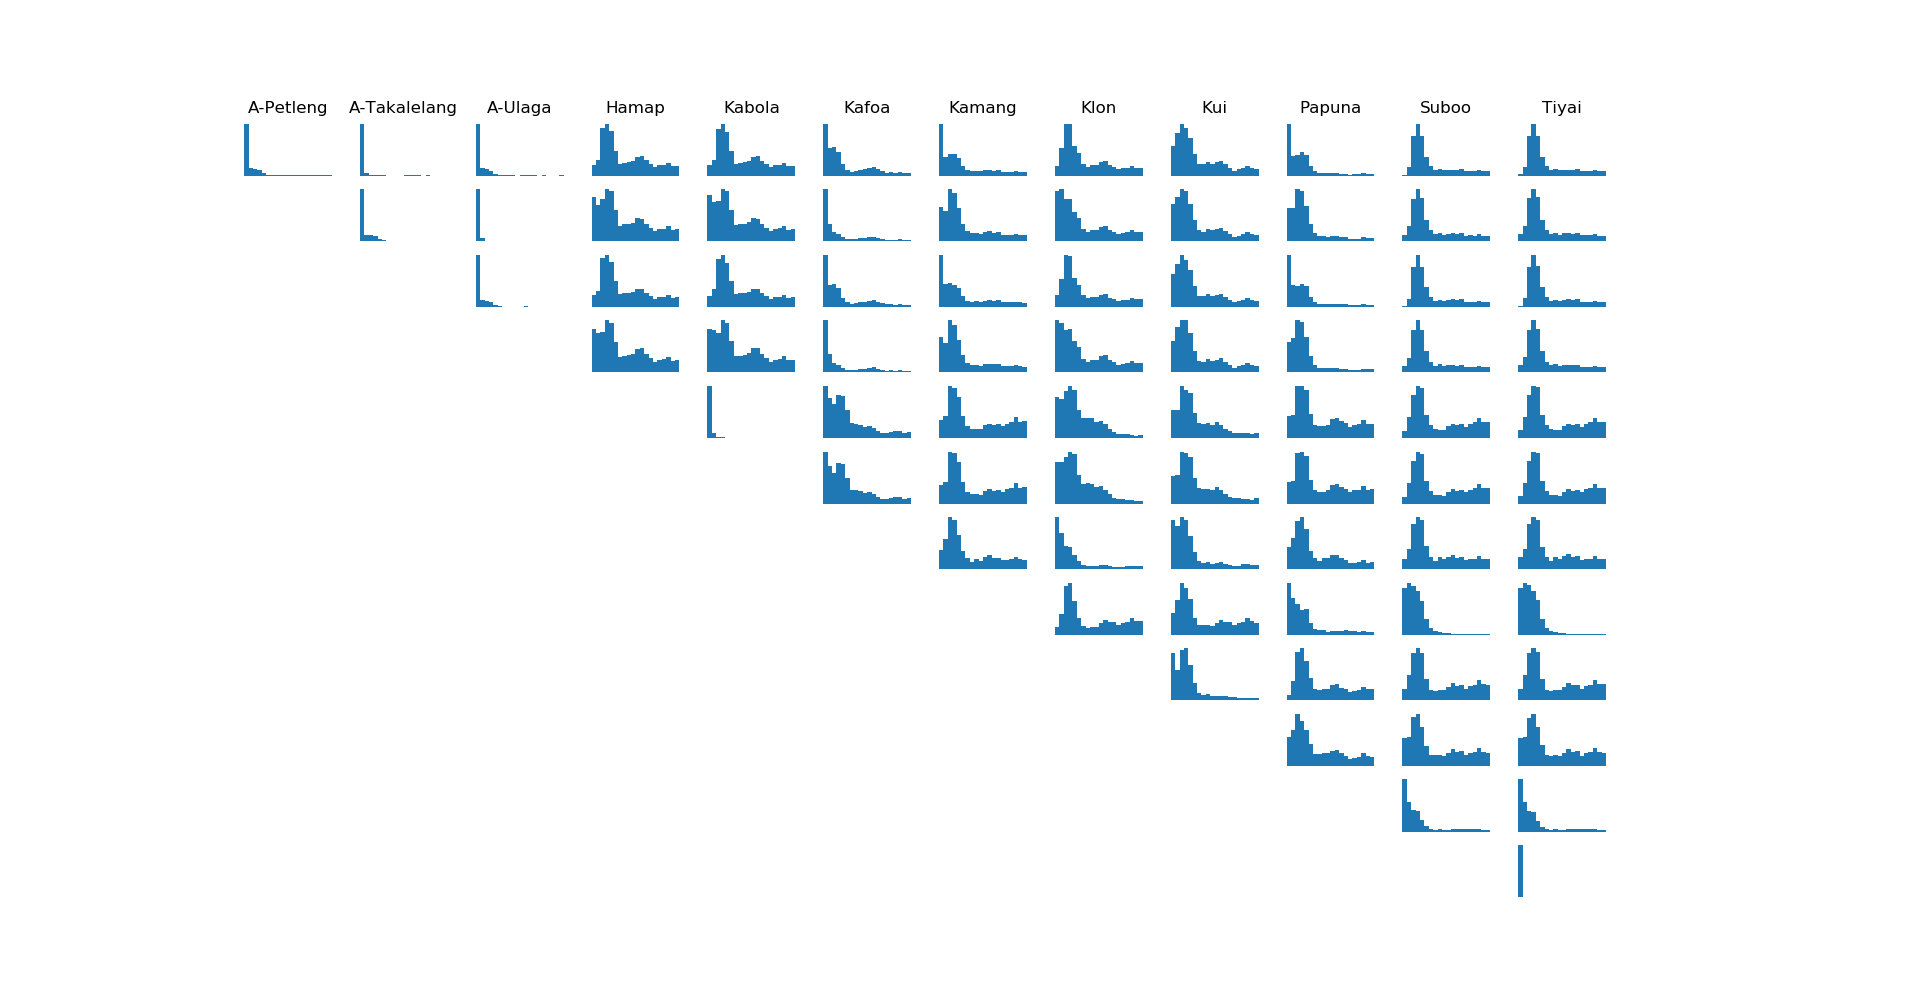
\includegraphics[clip, trim=2.5cm 1.5cm 2.5cm 1.5cm, width=\textwidth]{pairwise_distances}
    \end{column}
  \end{columns}
\end{frame}
\begin{frame}{Results}
  SplitsNetwork from mean distances
  \includegraphics[width=\textwidth]{distances}
\end{frame}
\begin{frame}{Computer-\emph{assisted}?}
  Words that most often follow different trees
  \medskip
  \begin{columns}
    \begin{column}{0.5\textwidth}
      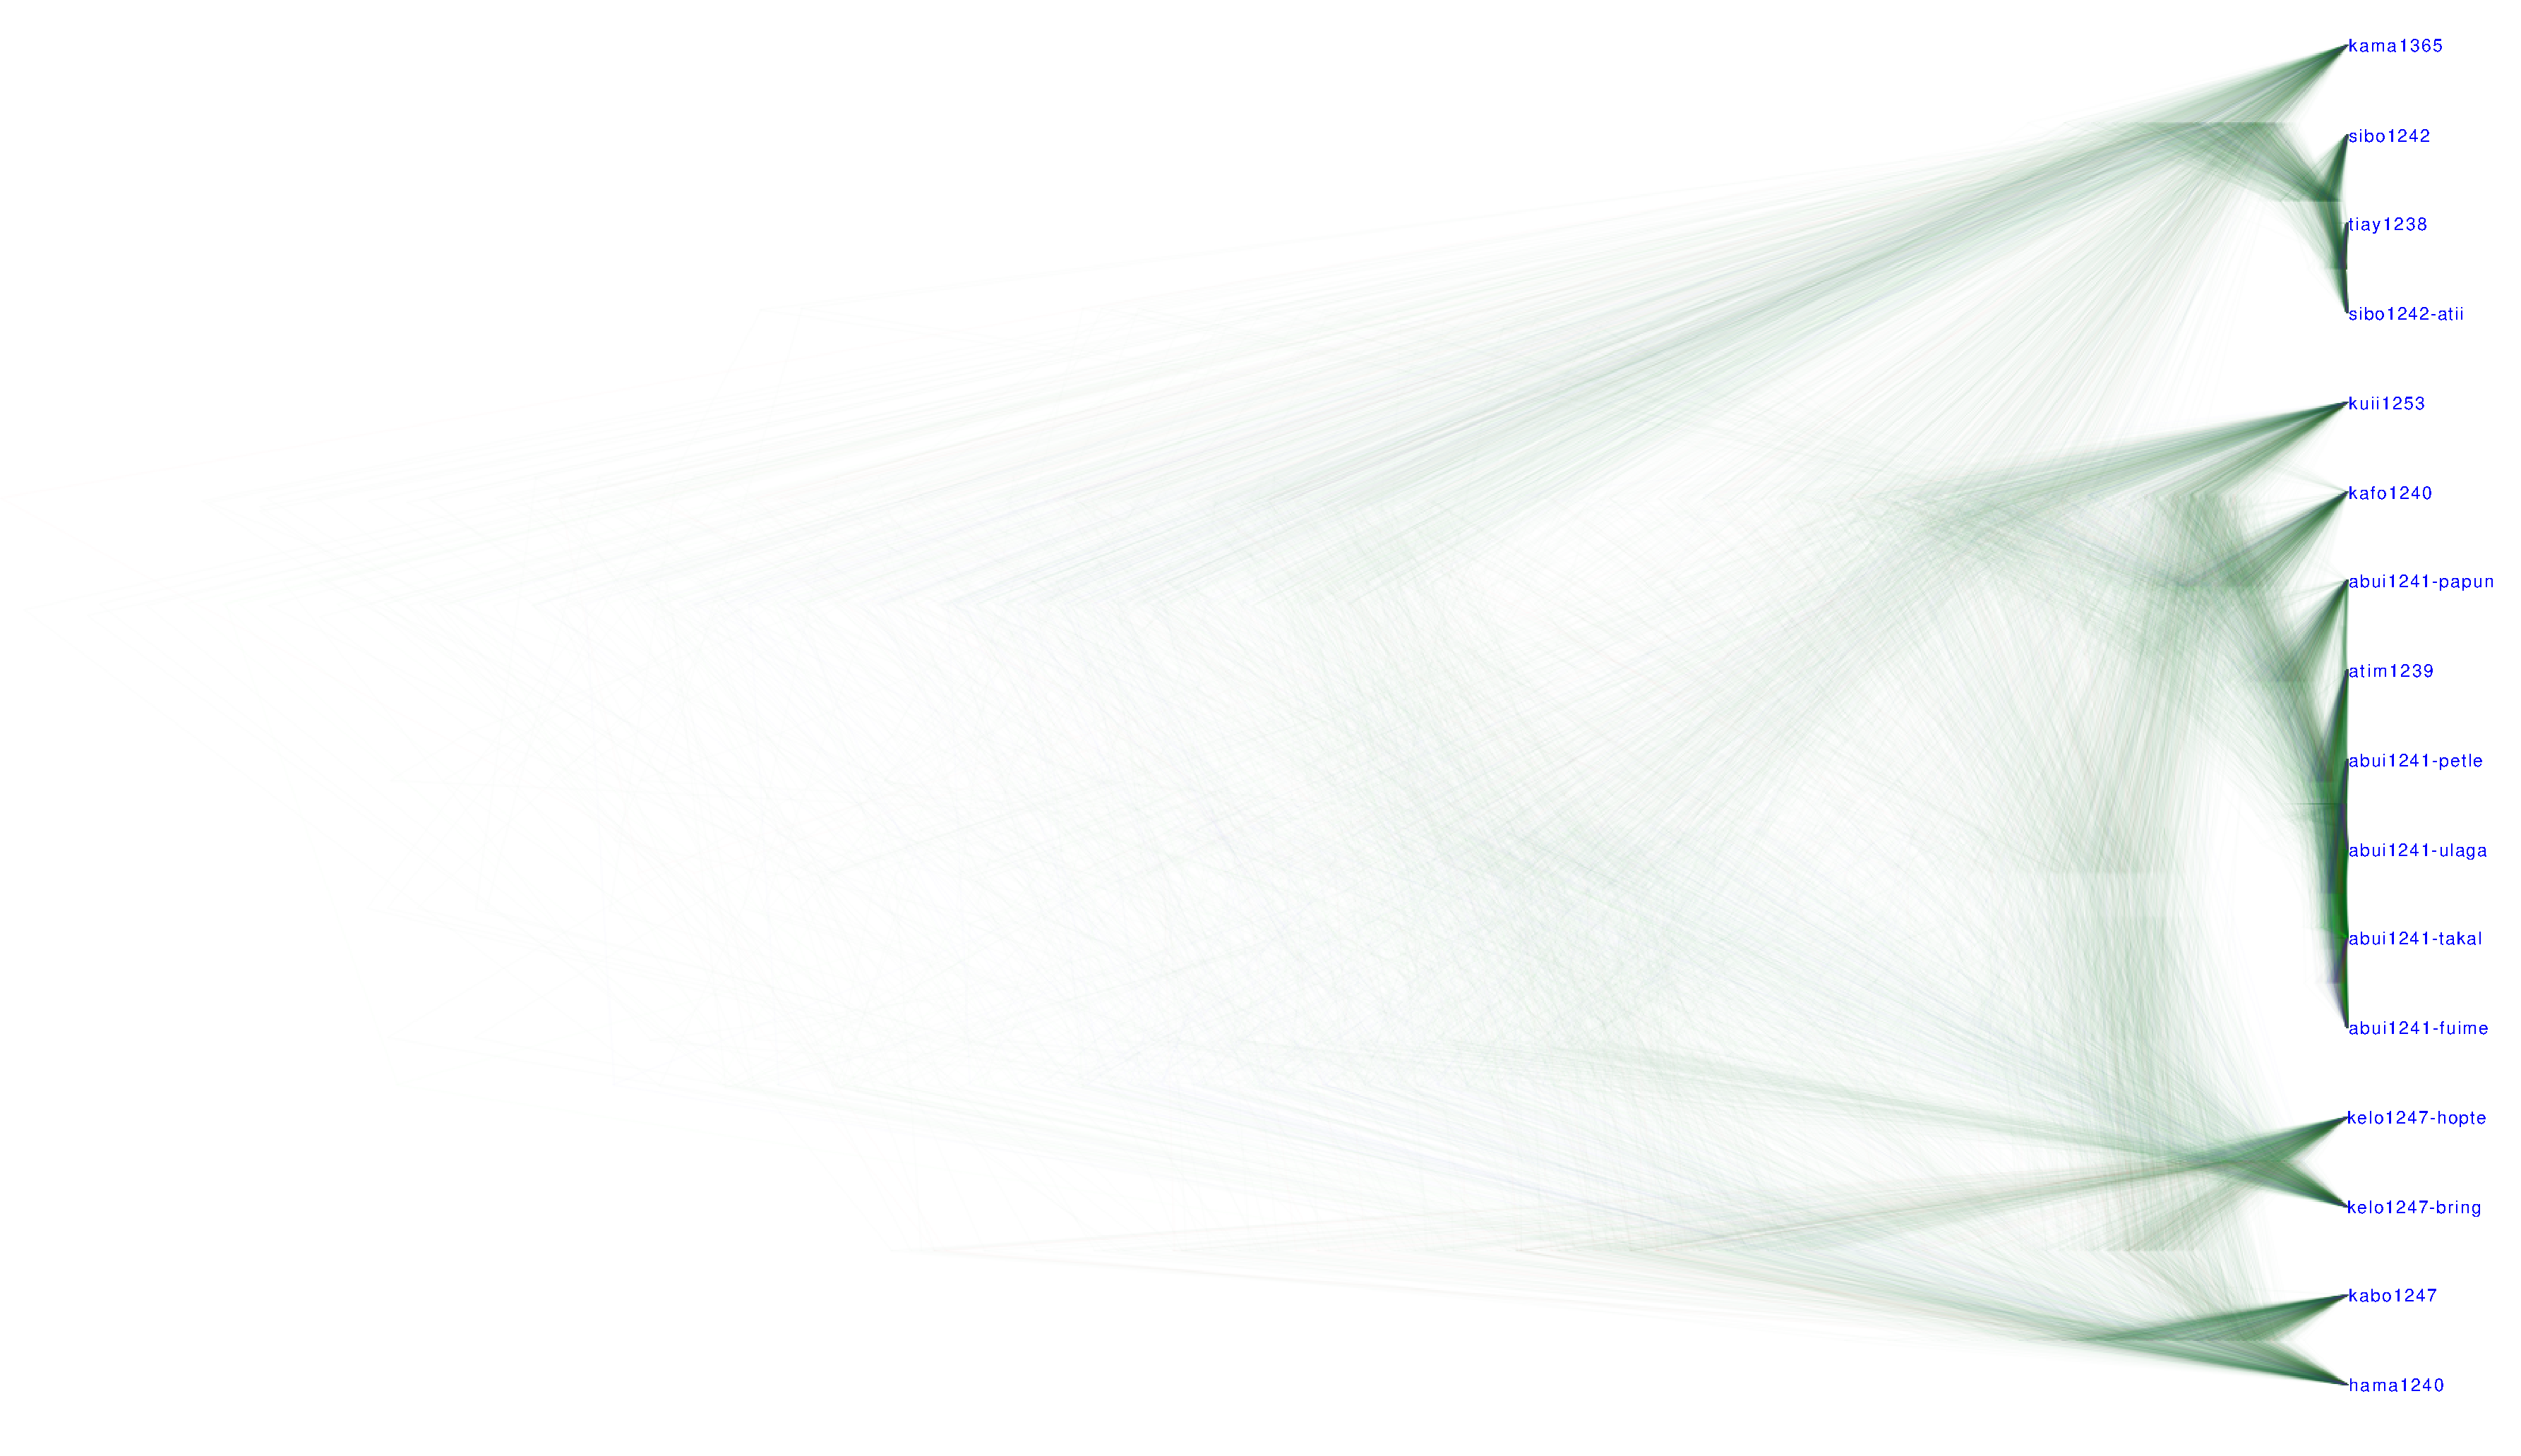
\includegraphics[clip, trim=10cm 1cm 0cm 1cm, width=\textwidth]{trees3.pdf}

      \footnotesize dark, water, to-stand, wing, to-search-for, fog, sweet, comb, nose, woman, to-spit, to-die, bad, star, fingernail
    \end{column}
    \begin{column}{0.5\textwidth}
      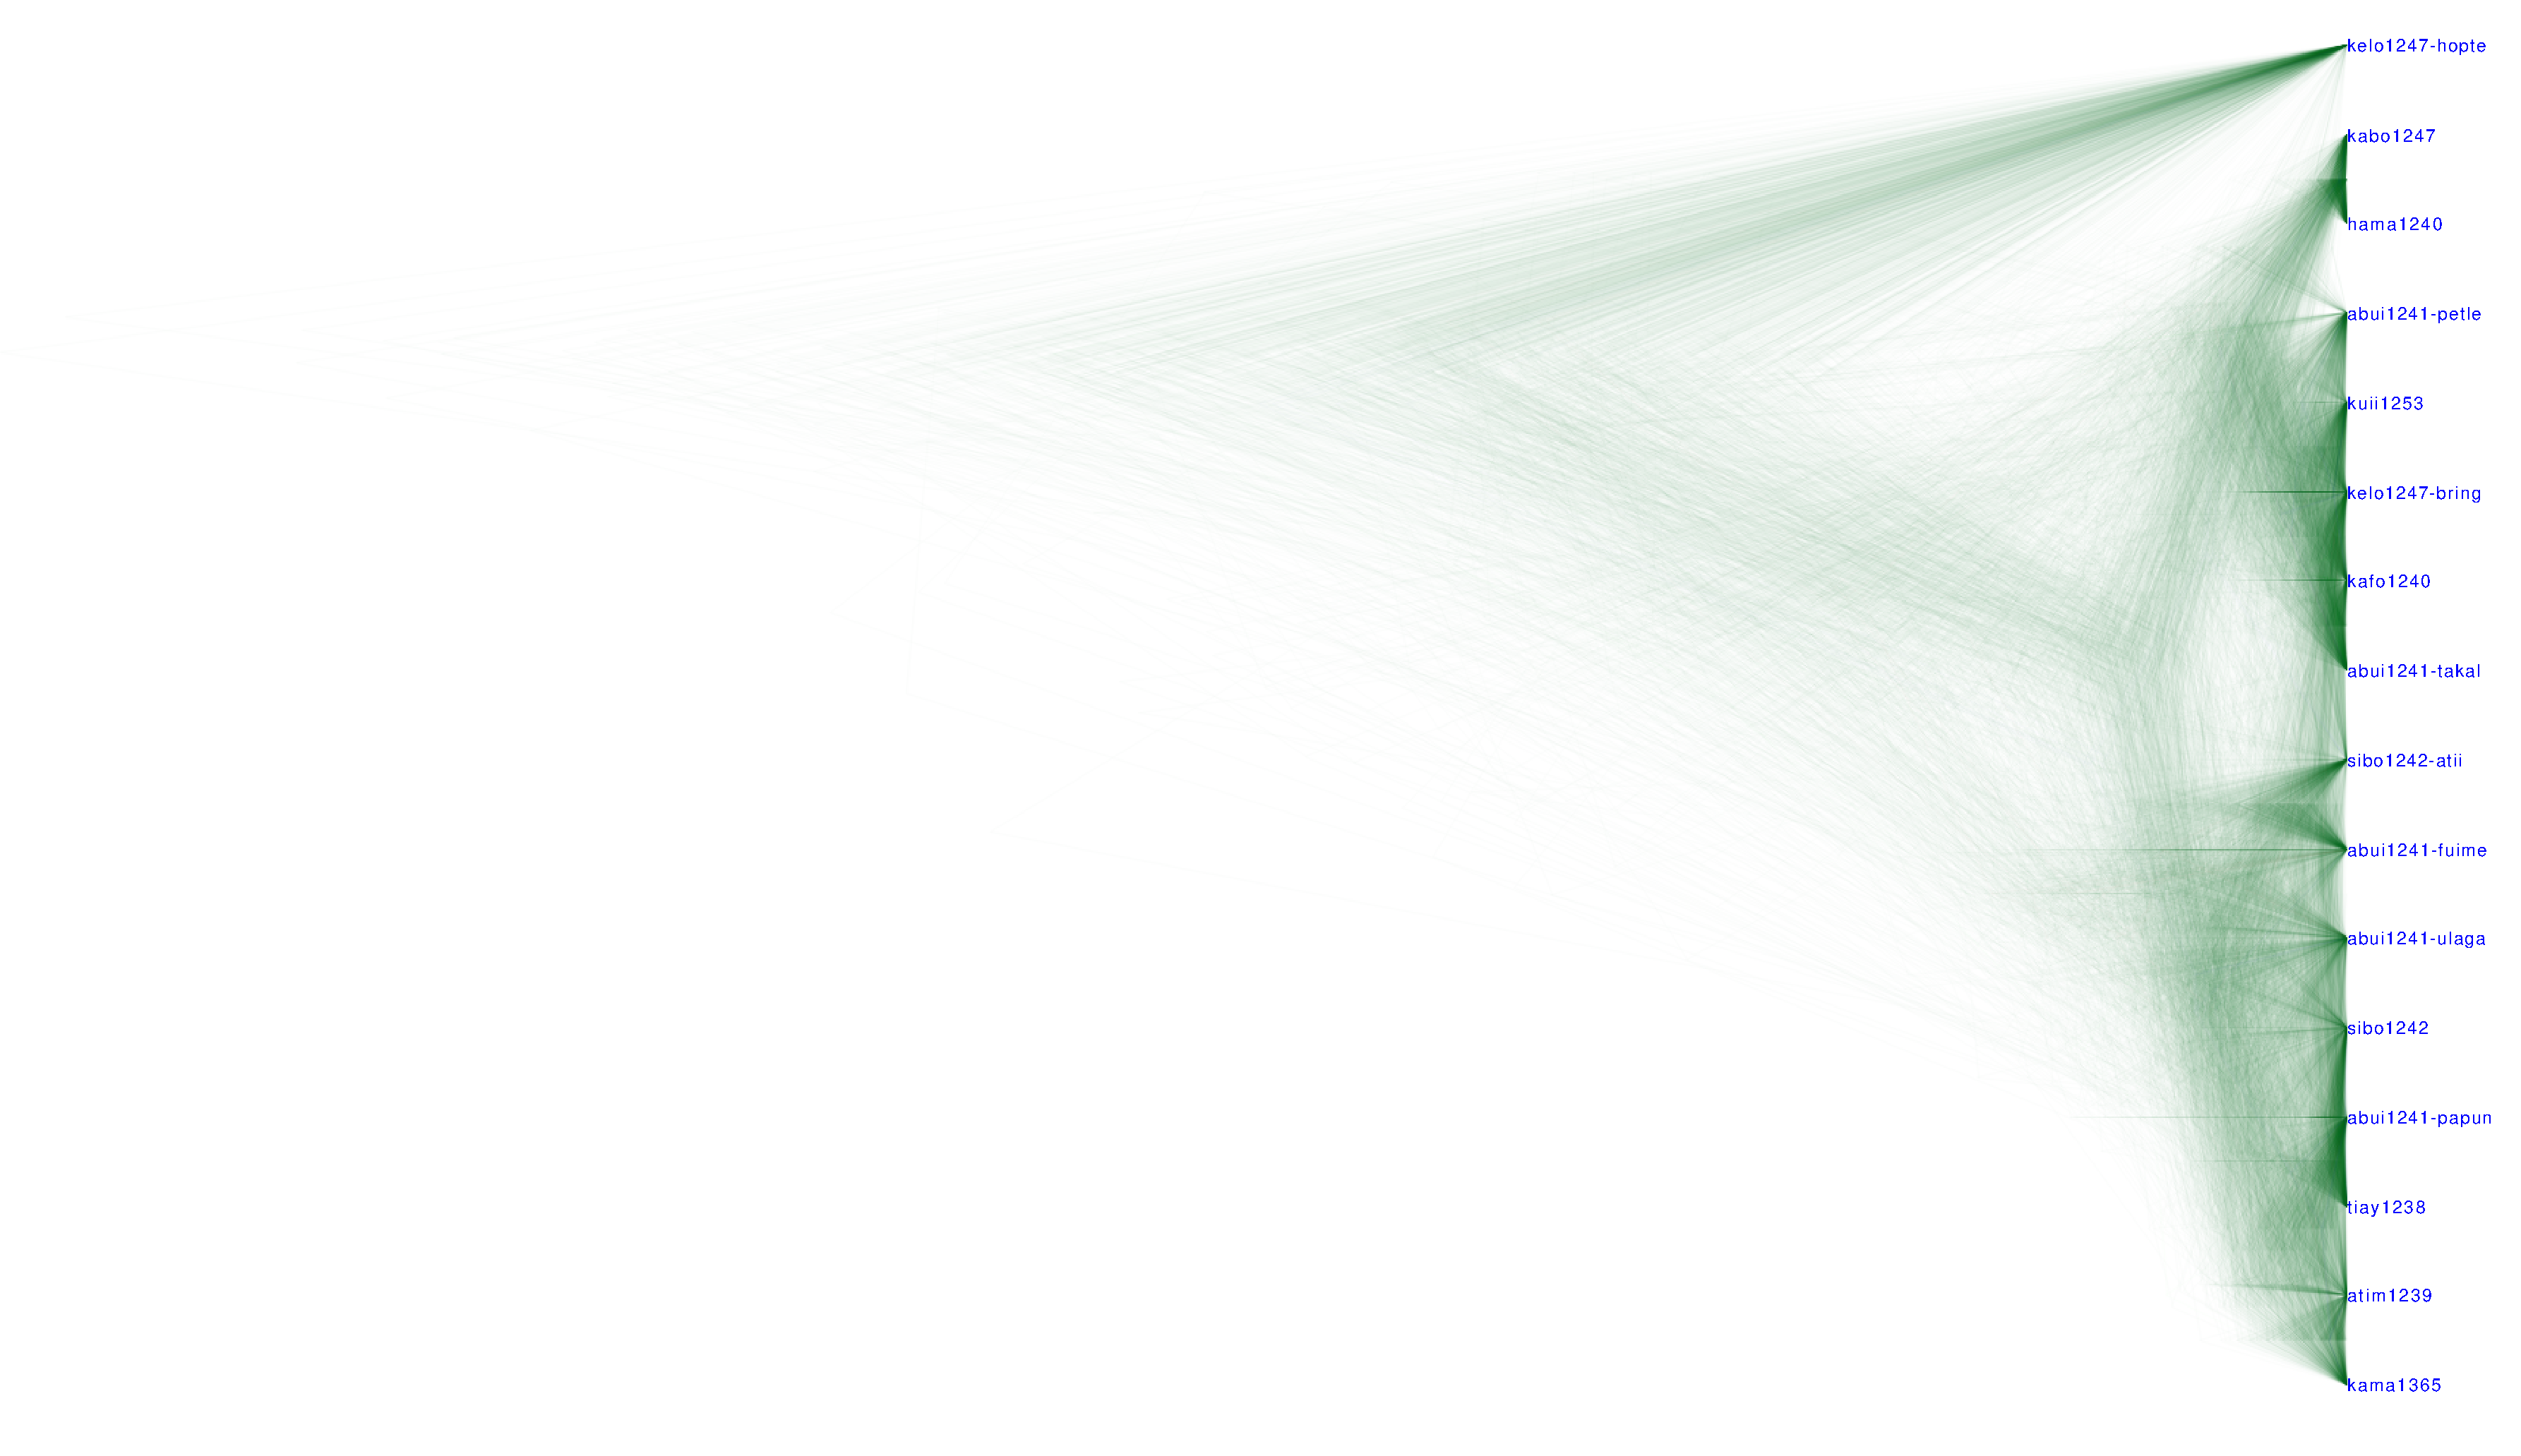
\includegraphics[clip, trim=10cm 1cm 0cm 1cm, width=\textwidth]{trees4.pdf}

      \footnotesize ripe, twenty-one, to-smell, fire, twenty, twelve, thirteen, to-buy, thirty, oven, eleven, sugar-palm, 3pl, horn, seventy
    \end{column}
  \end{columns}

  \medskip
  Candidates for informative vs. uninformative concepts?
\end{frame}
\section{Discussion}
\begin{frame}{Summary}
  \begin{itemize}
  \item Abui \& neighbours (Kafoa, Papuna!) are inferred with a lot of contact signal
  \item No a-priori borrow detection, maybe even find strata in the lexicon
  \item Start adding networks to our toolbox, solve outstanding issues
    \begin{itemize}
    \item Modeling
    \item Technology
    \item Validation
    \item Visualization
    \end{itemize}
  \end{itemize}
\end{frame}
\end{document}
%%% Local Variables:
%%% TeX-engine: luatex
%%% End: 